

\titleformat{\chapter}[block]
{\filcenter\bfseries\Huge}
{\xrfill[0.4ex]{5pt}\ \thechapter.\ \xrfill[0.4ex]{5pt}}
{0pt}
{\xrfill[0.4ex]{5pt}\ \MakeUppercase{#1}\ \xrfill[0.4ex]{5pt}}


\titleformat{\chapter}[block]
{\filcenter\bfseries\Huge}
{\xrfill[0.4ex]{5pt}\ \thechapter.\ \xrfill[0.4ex]{5pt}}
{0pt}
{\xrfill[0.4ex]{5pt}\ \MakeUppercase{#1}\ \xrfill[0.4ex]{5pt}}


\chapter*{Chapter 1}
\markboth{Chapter 1: Preliminary study}{1 Preliminary study} %pour afficher l'entete
\addcontentsline{toc}{chapter}{1 Preliminary study}




\setcounter{chapter}{1}


\etocsettocstyle{\subsection*{Plan}}{}
\vspace{0.25cm}

\setcounter{tocdepth}{1}
\headrule{
\vspace{0.5cm}

\begin{center}
    \textsc{\textbf {\Huge Preliminary study}} 
\end{center}
}
\headrule


\localtableofcontents
\newpage


%\end{chapter1}
\section*{Introduction}
Through this chapter we'll have a clear vision about the host company , its filed of activity  and its artifacts beside the global context of my internship .Also in this chapter we'll shed light on the encountered problematic and some existing solutions in the market and their limitations, then we'll have a comparative study of project management methodologies to come up with a suitable one for the needs of this project .


\section{Presentation of host organization}

This internship took place at Business Intelligence For Telecommunication, a TIC (Information and Communication Technology) company, founded in 2010, provides reliable and comprehensive solutions for the study, control, and monitoring of the quality of service of cellular networks. BI4T operates in various parts of the value chain of TIC (Information and telecommunication Technology) such as radio, architectural design, and software development. located at Tunis.

It was done over an extended  period of four months, from 1\textsuperscript{st}
February 2024 to 31 May 2024.

\begin{figure}[H]
    \centering
    
\includegraphics[height=4.5cm]{images/chap1/LOGO_BI4T.png}
    \caption{BI4T Logo} \cite{BI4T}
    \label{fig:enter-label}
\end{figure}

\section{BI4T legacy}
Throughout a span of 14 years BI4T has gained an understanding of the frameworks and market dynamics in the telecommunications sector. This vast experience has allowed them to navigate the realm of compliance while also leveraging emerging market trends. A standout accomplishment, on this journey is the creation of the QoS Tracker, a tool that transforms how customers monitor and manage telecommunications processes. With its range of features the QoS Tracker not meets but surpasses our clients requirements offering unmatched insights, into the service quality delivered by telecommunications networks.

\begin{figure}[H]
    \centering
    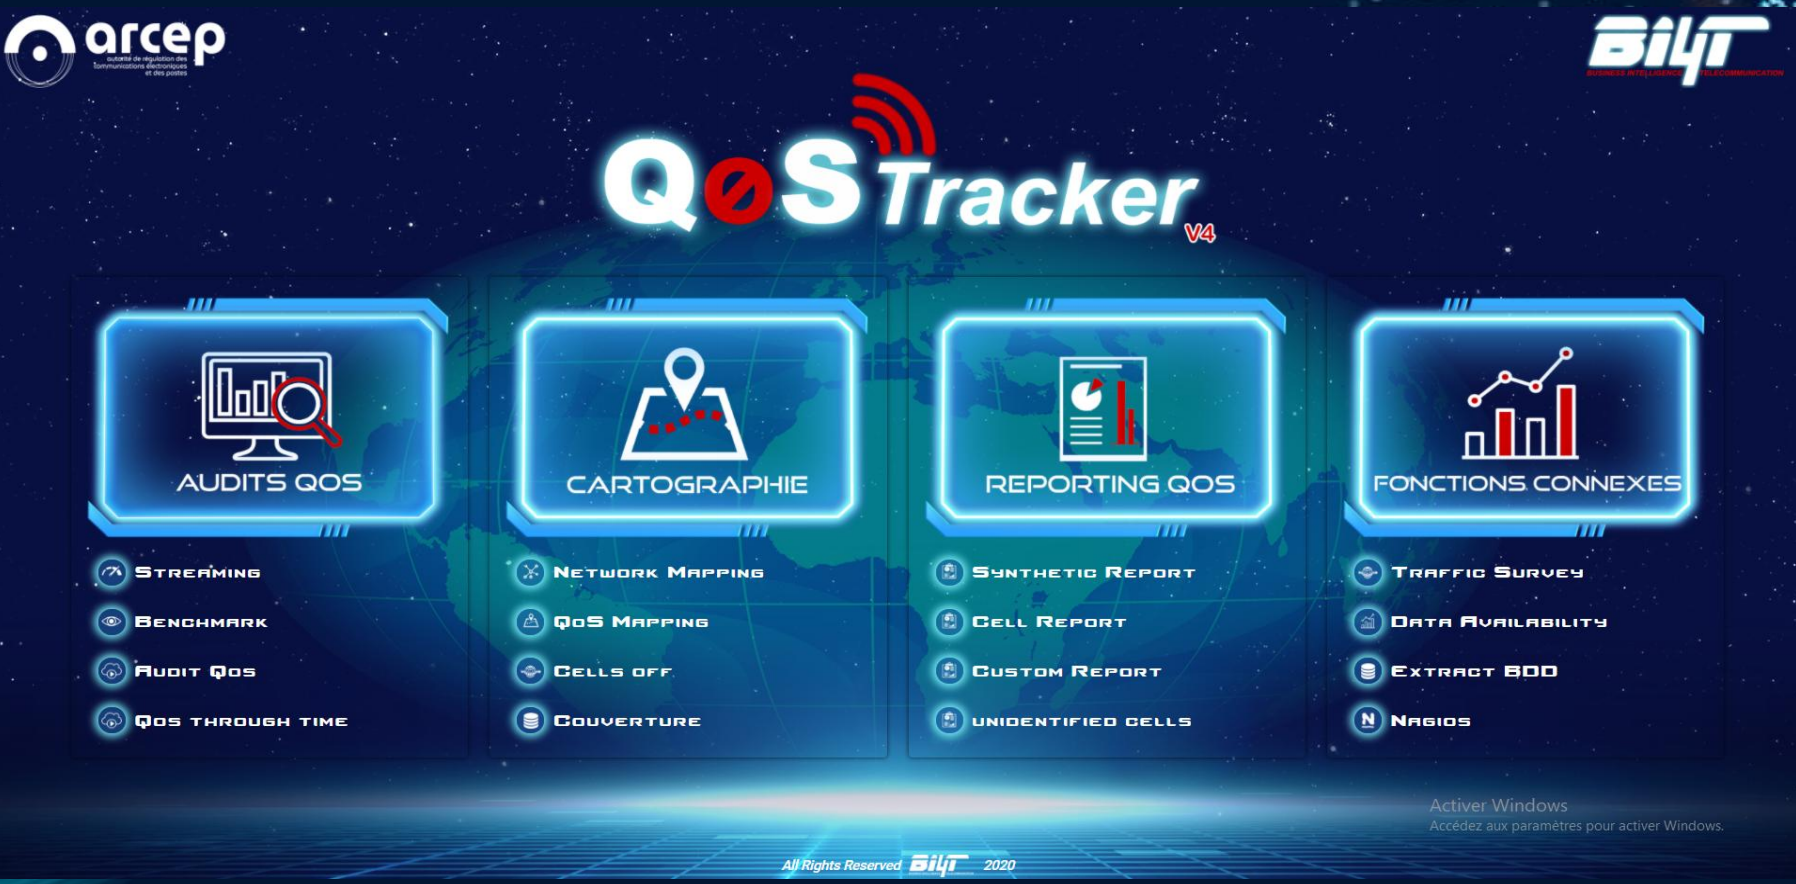
\includegraphics[height=8cm]{images/chap1/QoStrackerV4.png}
    \caption{QoS tracker interface}
    \label{fig:enter-label}
\end{figure}
\begin{figure}[H]
    \centering
    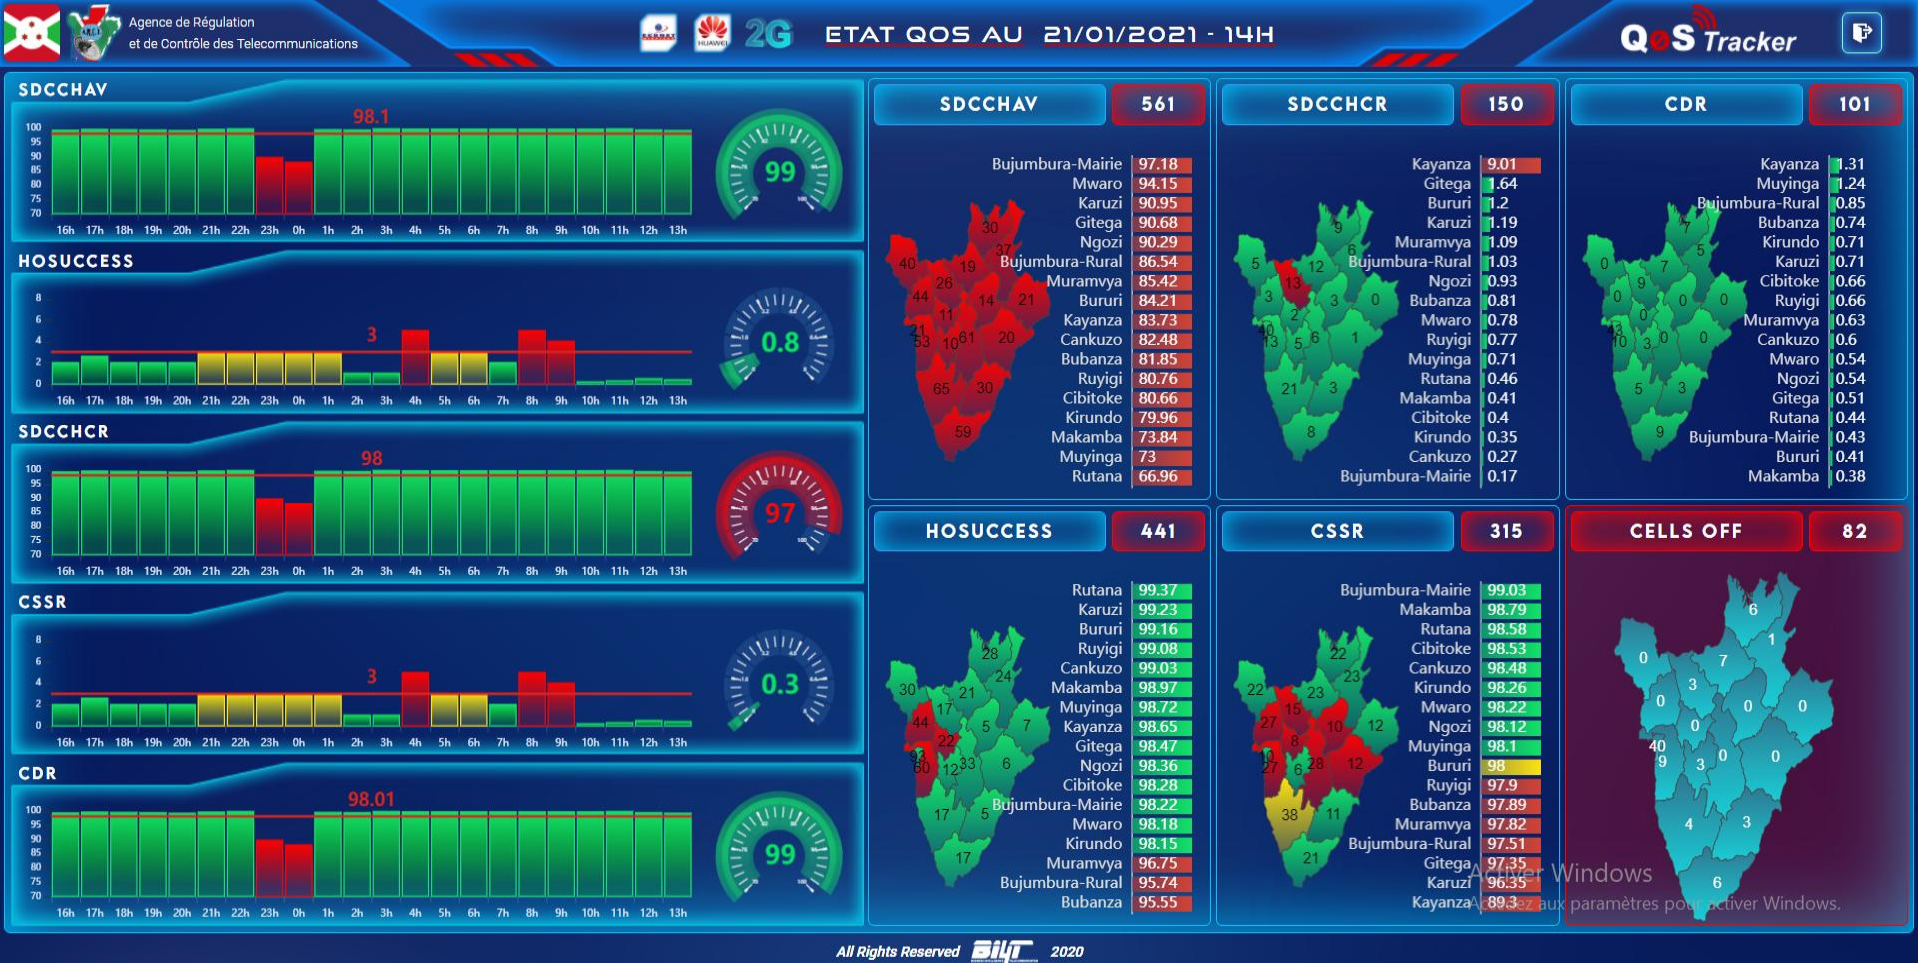
\includegraphics[height=8cm]{images/chap1/QoStrackerV4_1.png}
    \caption{QoS tracker interface}
    \label{fig:enter-label}
\end{figure}




\section{Telecommunication regulation process}
Our contemporary landscape of electronic communication is imbued with layers of significance and confidentiality, rendering it invaluable in its essence. Understanding the weight of this reality, governments worldwide have instituted a comprehensive regulatory regime to oversee telecommunication companies and operators. Through the enactment of laws and the establishment of regulatory bodies, these governments seek to create a framework that balances the imperatives of security, privacy, and accessibility. The power of monitoring vested in these regulatory entities serves as a linchpin for ensuring compliance and upholding the integrity of the telecommunication process.
As a two major axis of this regulation , governments instances often emphasize the importance of ensuring that users privacy is respected, as maintaining a fair level of quality of service (QoS) and quality of experience (QoE). 
% not done yet need one more img to describe the process + some points to describe each step
The result of this process is determined by the calculation of some KPI :
\begin{itemize}
    \renewcommand\labelitemi{\textbf{\Huge .}}
    \item  An OMC server collects raw data that contains some counter values from operator site and send them  to a DCS sever
    \item  Every DCS server organize the coming files in group based on equipment type and network generation then sends them to a dedicated server in the regulator site via a secure connection 
    \item The frontal servers then perform the processing and calculation of the provided counters based on a documentation given by the operator to have the final values of the KPIs 
    \item The frontal servers save raw data and aggregated data to the database 
    \item Web client consume the aggregated data to perform visualization and extract value from it 
    \end{itemize}

\begin{figure}[H]
    \centering
    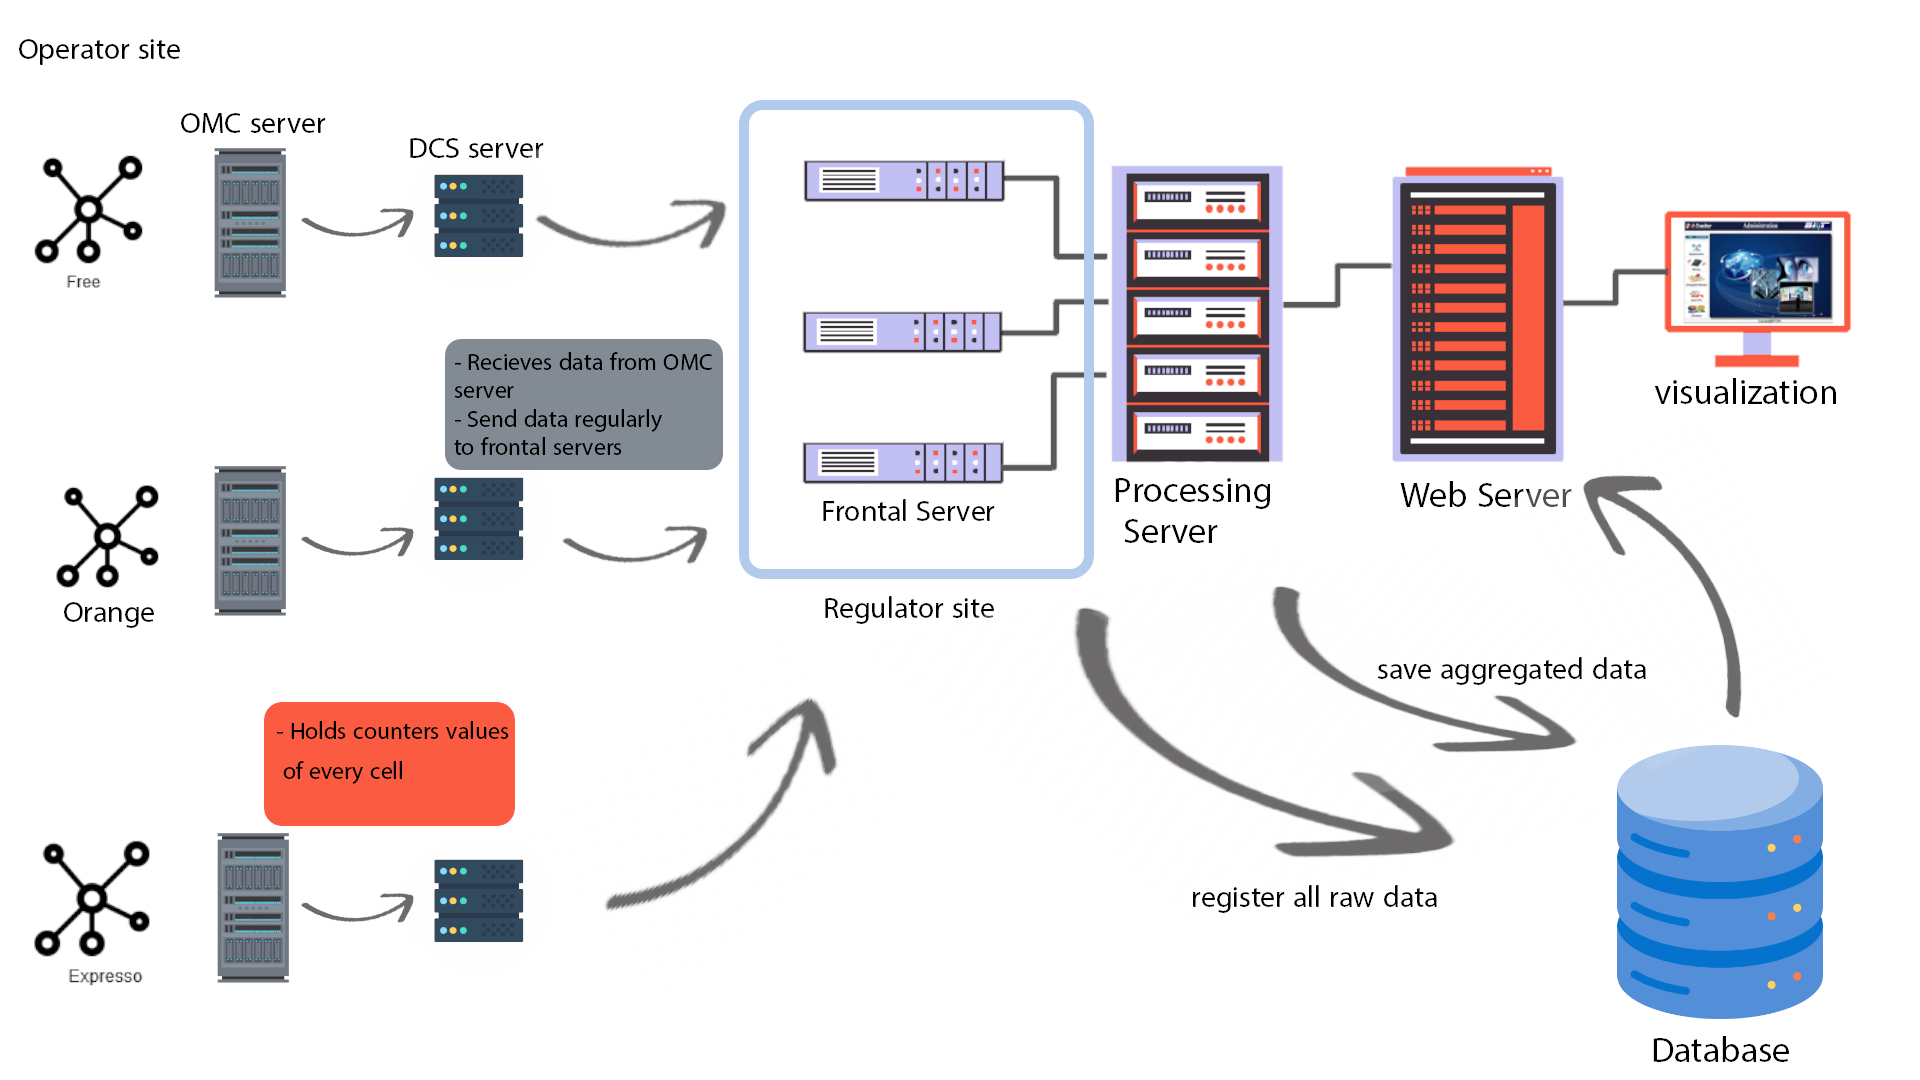
\includegraphics[height=10cm]{images/chap1/archi_1.png}
    \caption{Regulation process schema}
    \label{fig:enter-label}
\end{figure}






\section{Problematic}
BI4T offers a specialized software package tailored for professional utilization, which inherently relies on the expertise of regulatory technicians for its effective implementation. However, the absence of skilled subscribers poses a significant risk to its efficacy. In response to the imperative of transparency and efficient information dissemination, regulatory bodies frequently opt to complement their software package with a companion mobile application. This strategic choice aims to bridge potential gaps caused by subscriber absence. Our responsibility involves the development of this mobile channel, ensuring its accessibility and user-friendliness across all user demographics. Through this application, users gain access to a comprehensive repository of relevant information, facilitating the continuous monitoring of network conditions. Additionally, it serves as a platform for users to offer feedback and make inquiries, fostering a collaborative environment conducive to the enhancement of telecommunications services.


% \section{Proposed Solution}
\newpage
\section{Existing  Solutions}
A lot of companies have treated the quality of service tracking topic with applications such as:


\subsection{nPref speed test}
\textbf{nPerf}   brings you the best and the fullest mobile connection quality measurement tool up to 1 Gb/s speeds!

Full QoS test: In few seconds, test your bitrate speed, latency, browsing speed and video streaming quality on your mobile device.
Comparison function: Compare your results with those of others users and for each provider with a real time barometer.
Interactive map: Check network coverage and carriers performances in your area (in USA : AT\&T, Sprint, T-Mobile, Verizon Wireless).\cite{nPerf}
% \cite{https://play.google.com/store/apps/details?id=com.nperf.tester&hl=en&gl=US}.
\begin{figure}[H]
    \centering
    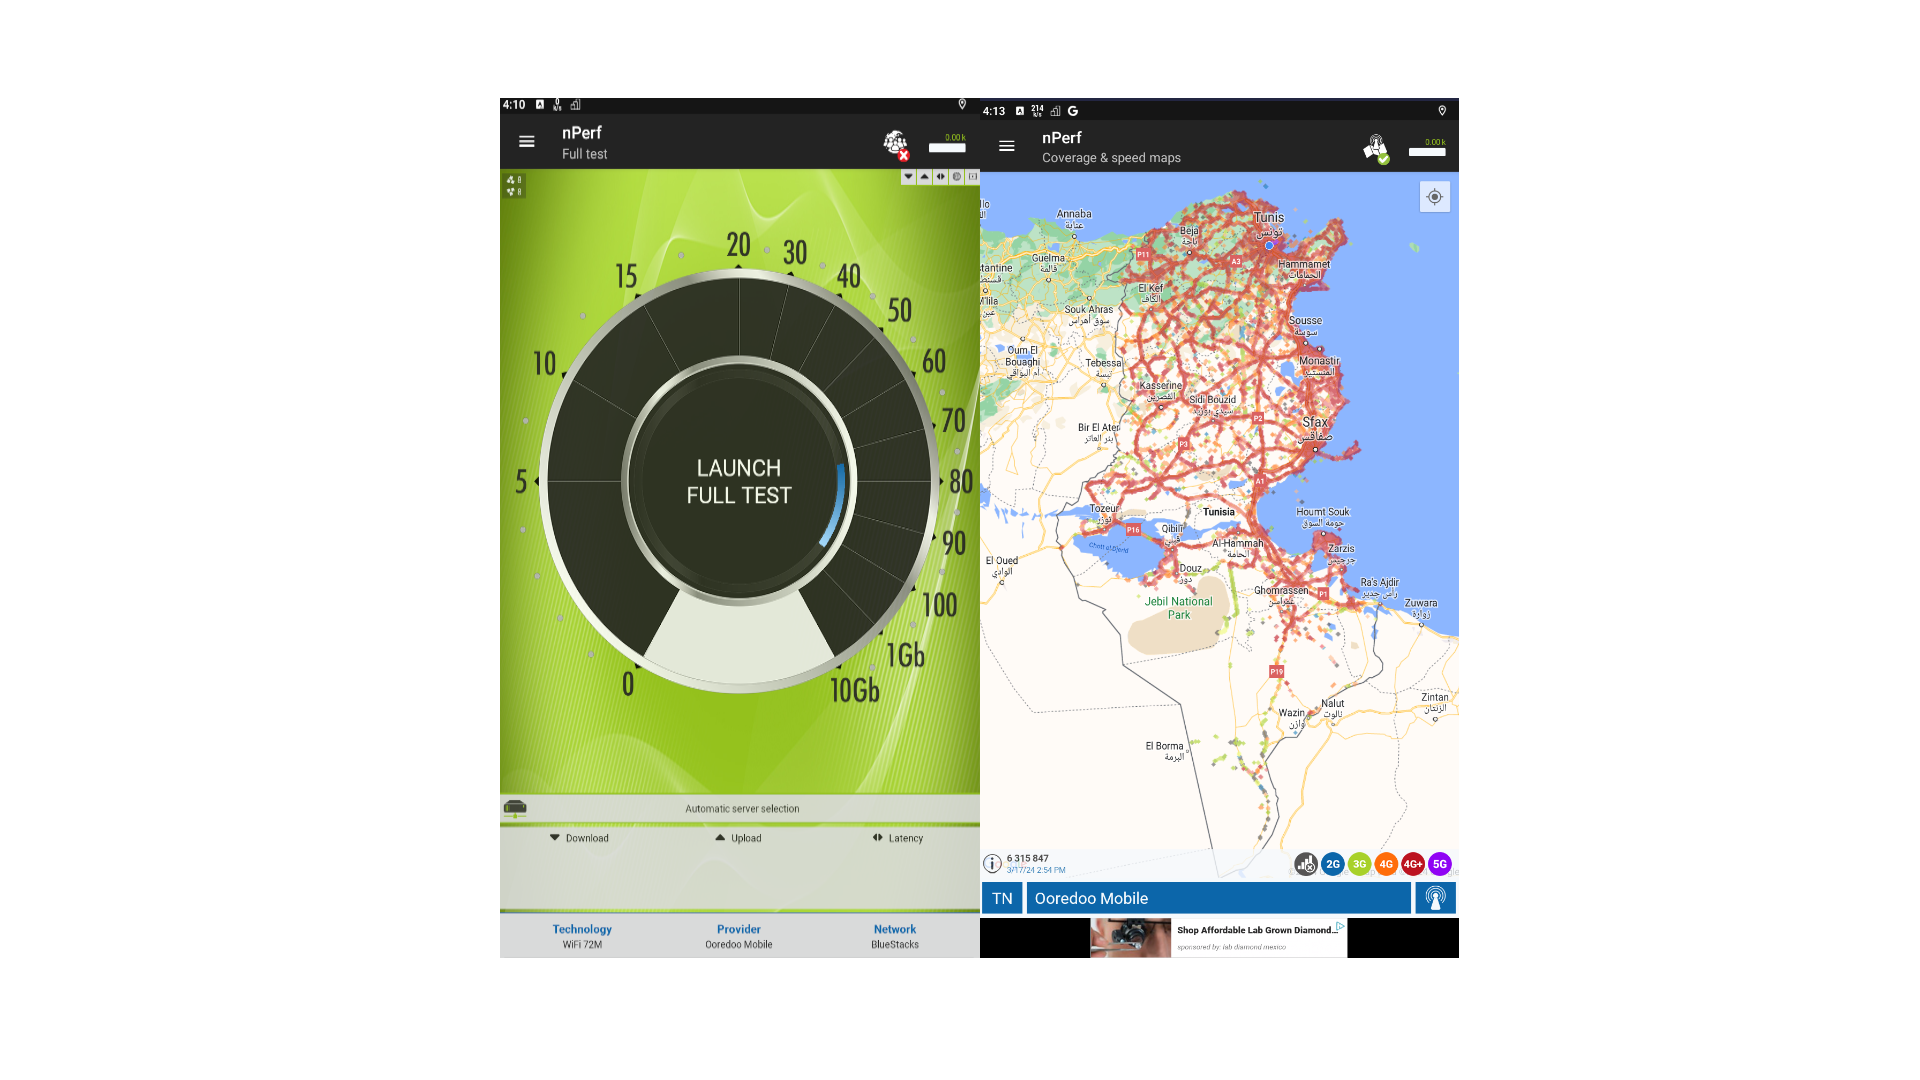
\includegraphics[height=12cm]{images/chap1/nPref.png}
    \caption{nPref speed test demo}
    \label{fig:enter-label}
\end{figure}
\textbf{nPref} mobile app comes up with :
\begin{itemize}
    \renewcommand\labelitemi{\textbf{\Huge .}}
    \item  Decent User Interface
    \item  Speed test section
    \item Coverage map 
  
\subsubsection*{Advantages}
\begin{itemize}
\renewcommand\labelitemi{\textbf{\Huge .}}
    \item Fullest mobile connection quality measurement tool up to 1 Gb/s speeds
    \item User friendly interface
\end{itemize} 

\subsubsection*{Disadvantages}
\begin{itemize}
\renewcommand\labelitemi{\textbf{\Huge .}}
    \item The data is often outdated 
    \item Without subscription user forced to see adds
    \item The data source in unknown
\end{itemize} 
\end{itemize}

% 2nd
\subsection{RfBenchmark}
\textbf{RfBenchmark}  Mobile application RFBENCHMARK allows measurements of radio coverage provided by mobile operator and testing of Internet Connection Quality for different Radio Access Technologies (RAN), such as: GSM, 3G, LTE, WIFI.\cite{RFBenchmark}
% \cite{https://rfbenchmark.com/en/application-2/}.
\begin{figure}[H]
    \centering
    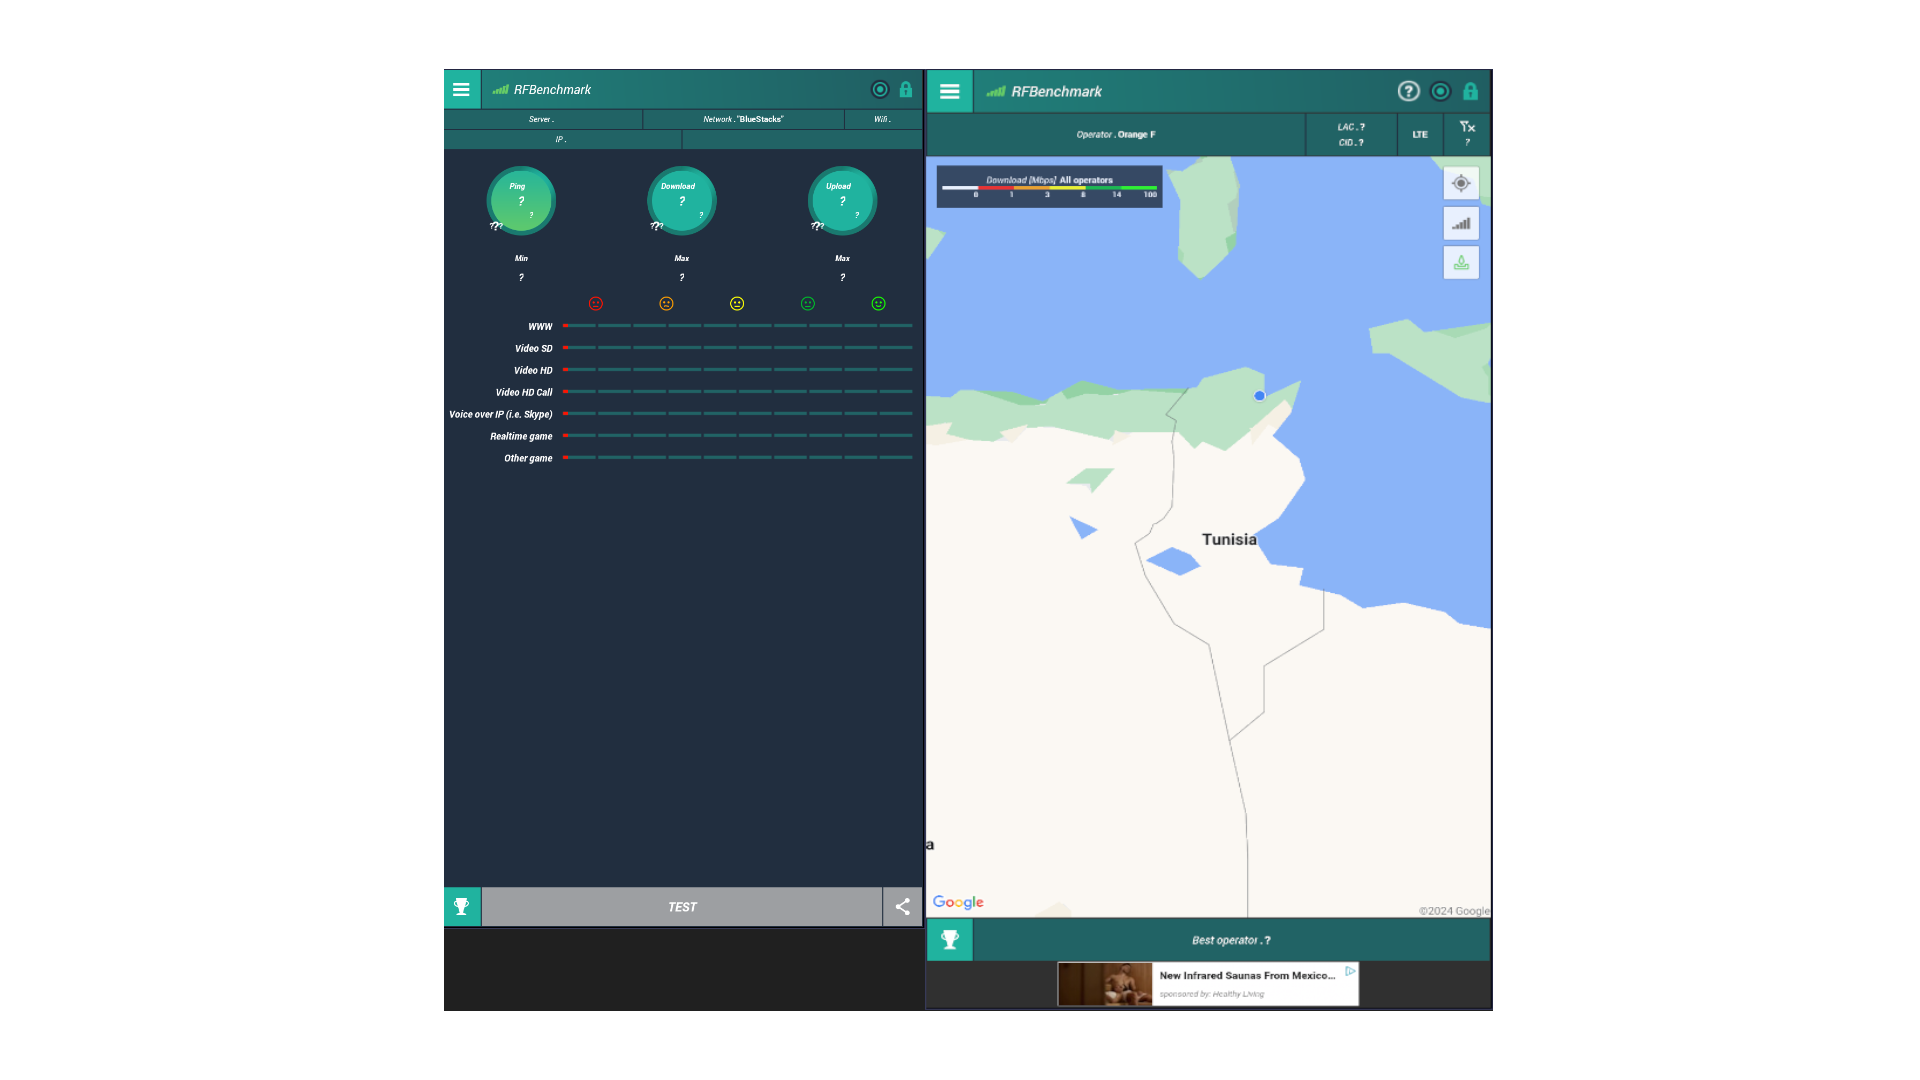
\includegraphics[height=10cm]{images/chap1/RFBenchmark.png}
    \caption{RfBenchmark demo}
    \label{fig:enter-label}
\end{figure}
\textbf{RfBenchmark} mobile app comes up with :
\begin{itemize}
    \renewcommand\labelitemi{\textbf{\Huge .}}
    \item  Speed test section
    \item Coverage map 
    \item Search functionality 
    \item Operators and networks ranking
  
\subsubsection*{Advantages}
\begin{itemize}
\renewcommand\labelitemi{\textbf{\Huge .}}
    \item Very detailed performance test
    \item User can give feedback
\end{itemize} 

\subsubsection*{Disadvantages}
\begin{itemize}
\renewcommand\labelitemi{\textbf{\Huge .}}
    \item The data is often outdated  
    \item Coverage map is not available in all counties 
    \item The data source in unknown
    \item In app adds 
    \item Complex user interface
\end{itemize} 
\end{itemize}

\section{Proposed Solution}
After planning and, in depth market research the BI4T team has introduced a new mobile app idea aimed at improving telecommunication services tracking  for individuals . This innovative concept is set to transform Quality of Service (QoS) monitoring by overcoming market challenges and providing users with options. The app is built on a foundation of both non practical needs forming the basis of its creation.
This application will let the user to :
\begin{itemize}
\renewcommand\labelitemi{\textbf{\Huge .}}
    \item Perform some tests on his network(upload and download speed and latency)  
    \item Save test's result 
    \item View  statistics and charts based on his tests
    \item View a leader-board of  best operators 
    \item View a coverage and speed map of his country
    \item Submit  feedback to the authorities and receive responses from them .
\end{itemize} 



\section{Project management Methodology}

Project management methods are essential, for carrying out projects in industries. They offer organized structures and guidelines that assist teams in planning, executing and overseeing projects from start to finish efficiently. By using these methods companies can improve project results reduce risks allocate resources better and deliver projects on time and within budget. Additionally it is important to recognize the distinctions, between project management methods to choose the appropriate approach based on project needs, team interactions and organizational goals.

\subsection{Comparative study of project management methodologies }
In the following table we'll have a comparison between widely used methods 
\begin{table}[H]
    % \centering
    % \renewcommand{\arraystretch}{2}
   
   \begin{tabular}{|p{0.15\textwidth}|p{0.20\textwidth}|p{0.13\textwidth}|p{0.14\textwidth}|p{0.25\textwidth}|p{0.1\textwidth}|}
   \hline
   
   Methodology & Core Ideas & Flexibility & Adaptability & Stakeholder Involvement & Iterative  \\ \hline

Waterfall & Sequential process with distinct phases (Requirements, Design, Implementation, Testing, Deployment). & Low & Low & Limited involvement primarily at the beginning and end of the project. & No \\ \hline

Agile & Iterative approach focusing on incremental delivery, collaboration, and flexibility. & High & High & Continuous involvement through active participation in iterations and feedback loops. & Yes \\ \hline

Scrum & Agile framework emphasizing small, cross-functional teams (Scrum Teams) working in short iterations (Sprints). & Moderate & Moderate & High involvement through roles like Product Owner, Scrum Master, and Development Team. & Yes \\ \hline

Kanban & Lean method focusing on visualizing work, limiting work in progress (WIP), and optimizing flow. & High & High & Moderate involvement, with stakeholders visualizing and managing work through Kanban boards. & Yes \\ \hline

Lean & Focuses on eliminating waste, maximizing customer value, and continuous improvement. & High & High & High involvement through value stream mapping and continuous improvement cycles. & Yes \\ \hline

\end{tabular}
    % \caption{Caption}
    % \label{tab:my_label}
     \setlength{\abovecaptionskip}{0.25cm} % Adjust the value as per your preference
    \caption{Comparison of Project Management Methodologies}
    \label{tab:Methodology_comp}
\end{table}

\subsection{SCRUM}
In our project, we have made a deliberate decision to incorporate the SCRUM methodology as our project management approach. This methodology acts as a reliable point of reference for resolving conflicts and overcoming obstacles throughout the project lifecycle. It is worth noting that SCRUM has gained high recognition and extensive adoption among successful teams in the industry.

One of the key reasons for SCRUM's popularity is the significant amount of flexibility and documentation it offers. The SCRUM framework allows us to adapt and respond to changing project requirements and priorities effectively. By breaking down the software development process into manageable sprints lasting one to four weeks, SCRUM enables us to deliver working and tested software components incrementally, ensuring that progress is continuously made.


\begin{figure}[H]
    \centering
    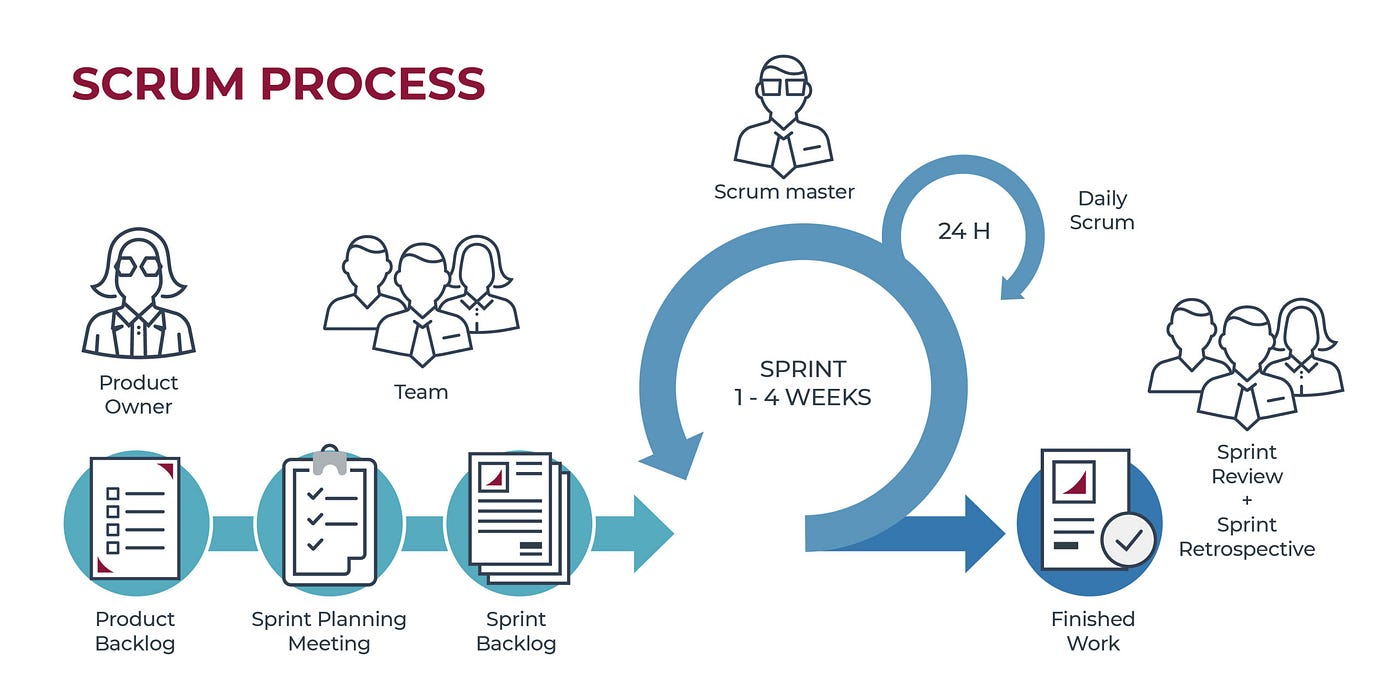
\includegraphics[height=9cm]{images/chap1/Scrum.jpg}
    \caption{Scrum Logo}
    \label{fig:enter-label}
\end{figure}

\subsection{How SCRUM works}
SCRUM follows an agile approach by breaking down project requirements into smaller, manageable chunks. This allows for iterative development and the delivery of incremental value. By treating requirements in this manner, SCRUM promotes flexibility, and accurate planning, resulting in higher client satisfaction and successful project outcomes. It allows for immediate feedback and adjustments, resulting in a higher level of client satisfaction.
This smooth workflow is attended thanks to some layers of abstraction given by SCRUM creators to separate and well define the project corner stones !

\subsection{Ceremonies}
SCRUM includes various ceremonies or meetings to facilitate collaboration and communication
\begin{itemize}
\item \textbf{Sprint Planning}: A meeting where the team determines which backlog items will be addressed in the upcoming sprint.
\item \textbf{Daily Scrum}: A brief daily meeting for the Development Team to synchronize their work, discuss progress, and identify any obstacles.
\item \textbf{Sprint Review}: A meeting at the end of each sprint where stakeholders provide feedback on the completed work and potentially adjust project priorities.
\item \textbf{Sprint Retrospective}: A reflection session where the team identifies strengths and areas for improvement in their process and teamwork for future sprints.
\end{itemize}
\subsection{Artifacts}

SCRUM also incorporates essential artifacts to have a clear version of the project state
\begin{itemize}
\item \textbf{Product Backlog}: A prioritized list of features, functionalities, and changes that need to be implemented in the project.
\item \textbf{Sprint Backlog}: A subset of items selected from the Product Backlog for a specific sprint, outlining the work to be completed.
\item \textbf{Increment}: The sum of all the completed Product Backlog items during a sprint, resulting in a potentially shippable product.
\end{itemize}

\subsection{Actors}
SCRUM involves specific actors or roles within the team to split workload and share responsibilities 
\begin{itemize}
\item \textbf{Product Owner}: The individual responsible for managing and prioritizing the Product Backlog, ensuring that the team focuses on delivering the most valuable features.
\item \textbf{Development Team}: A self-organizing group of professionals responsible for delivering the product increment during each sprint.
\item \textbf{Scrum Master}: The facilitator of the SCRUM process, ensuring that the team adheres to the framework and removing any impediments that hinder progress.
\end{itemize}
\vspace{0.5cm}
\section{Modeling language}
A modeling language serves as an standardized formal means to depict and explain systems, processes or ideas. It offers a collection of guidelines and symbols for crafting representations that illustrate the components, connections and actions, within a system or area. These languages find use across fields, like software development, system planning, data representation and business process depiction. Known examples of modeling languages encompass Unified Modeling Language (UML) Business Process Model and Notation (BPMN) Entity Relationship Diagram (ERD) and SysML (Systems Modeling Language).

\subsection{Unified modeling language (UML)}
UML is a modeling language used to depict systems in an object oriented way. It offers diagrams to illustrate behavior, interaction and structure. In class diagrams actors are depicted as classes. Entity relationship diagrams, in UML aid in simplifying database comprehension. They facilitate understanding of system elements and potential scenarios. Behavior and interaction diagrams portray behavior and message exchange. UML serves as an instrument, for representing systems designing databases and analyzing scenarios.

\begin{figure}[H]
    \centering
    
\includegraphics[height=4cm]{images/chap1/UML.png}
    \caption{Unified modeling language LOGO}
    \label{fig:enter-label}
\end{figure}

\subsection{Importance of UML}

Employing conceptual modeling during the development of information systems enables a more appropriate consideration of application needs and facilitates the abstract representation of certain aspects of physical and human systems.

\vspace{0.25cm}
\subsection*{Formal and Standardized Language}
\begin{itemize}
\renewcommand\labelitemi{\textbf{\Huge .}}
\item Ensures consistent use of UML elements for accurate representations.
\item Minimizes errors and improves development efficiency through common language.
\end{itemize}

\subsection*{Effective Communication Medium}
\begin{itemize}
\renewcommand\labelitemi{\textbf{\Huge .}}
\item Conveys complex ideas through clear visual representations.
\item Versatility and flexibility promote universal communication across teams.
\item Enables clear understanding between developers, designers, and stakeholders.
\end{itemize}

\subsection*{Tailored for Software Development}
\begin{itemize}
\renewcommand\labelitemi{\textbf{\Huge .}}
\item Designed specifically to specify, build, and document software systems.
\item Standardized notation balances design freedom with clear communication.
\item Combination of formality, standardization, communication, and modeling capabilities make UML ideal for many projects.
\item Visual diagrams offer diverse perspectives for comprehensive understanding of the software.
\end{itemize}
UML, a visual language, utilizes various diagrams. Each diagram offers a unique perspective on the software project, providing a comprehensive view of the system to be developed. These diagrams can be categorized based on whether they represent static aspects (structure) or dynamic aspects (behavior).


\begin{table}[H]
    % \centering
    % \renewcommand{\arraystretch}{2}

   \begin{tabular}{|p{0.3\textwidth}|p{0.60\textwidth}|}
   \hline
     
        \begin{center}
            \textbf{Static (structure)}
        \end{center} & 
        \begin{itemize}
            \renewcommand\labelitemi{\textbf{\Huge .}}

            \item Use cases  
            \item Classes  
            \item Components  
            \item Objects
            \item Deployment

        \end{itemize}  \\   \hline

        
        \begin{center}
            \textbf{Dynamic (behavioral)}
        \end{center} & 
        \begin{itemize}
            \renewcommand\labelitemi{\textbf{\Huge .}}
            
            \item  Sequences  
            \item  Activity  
            \item  State-transition  
            \item  Cooperation

        \end{itemize}
        \\   \hline

        
\end{tabular}
    \caption{UML Static \& Dynamic Diagrams }
    \label{tab:UML_diagrams_list}
     \setlength{\abovecaptionskip}{0.25cm}
\end{table}

In this project, we make use of two types of UML diagrams:

\vspace{0.25cm}

\begin{itemize}
\renewcommand\labelitemi{\textbf{\Huge .}}
\item Use case diagrams: These diagrams outline the functions of the application from the user's point of view.
\item Sequence diagrams: These diagrams illustrate the chronological and behavioral interactions between objects within the system.
\item Class diagrams: These diagrams depict the static structure of a system, including the classes, their attributes, methods, and the relationships between them.
\end{itemize}

\vspace{0.25cm}

\section{Terminologies}
As we delve into the project, it's helpful to clarify some important terminologies
\subsection{Business Intelligence}
Business intelligence combines business analytics, data mining, data visualization, data tools and infrastructure, and best practices to help organizations make more data-driven decisions. In practice, you know you’ve got modern business intelligence when you have a comprehensive view of your organization’s data and use that data to drive change, eliminate inefficiencies, and quickly adapt to market or supply changes. Modern BI solutions prioritize flexible self-service analysis, governed data on trusted platforms, empowered business users, and speed to insight
% \cite{https://www.tableau.com/learn/articles/business-intelligence}

\begin{figure}[H]
    \centering
    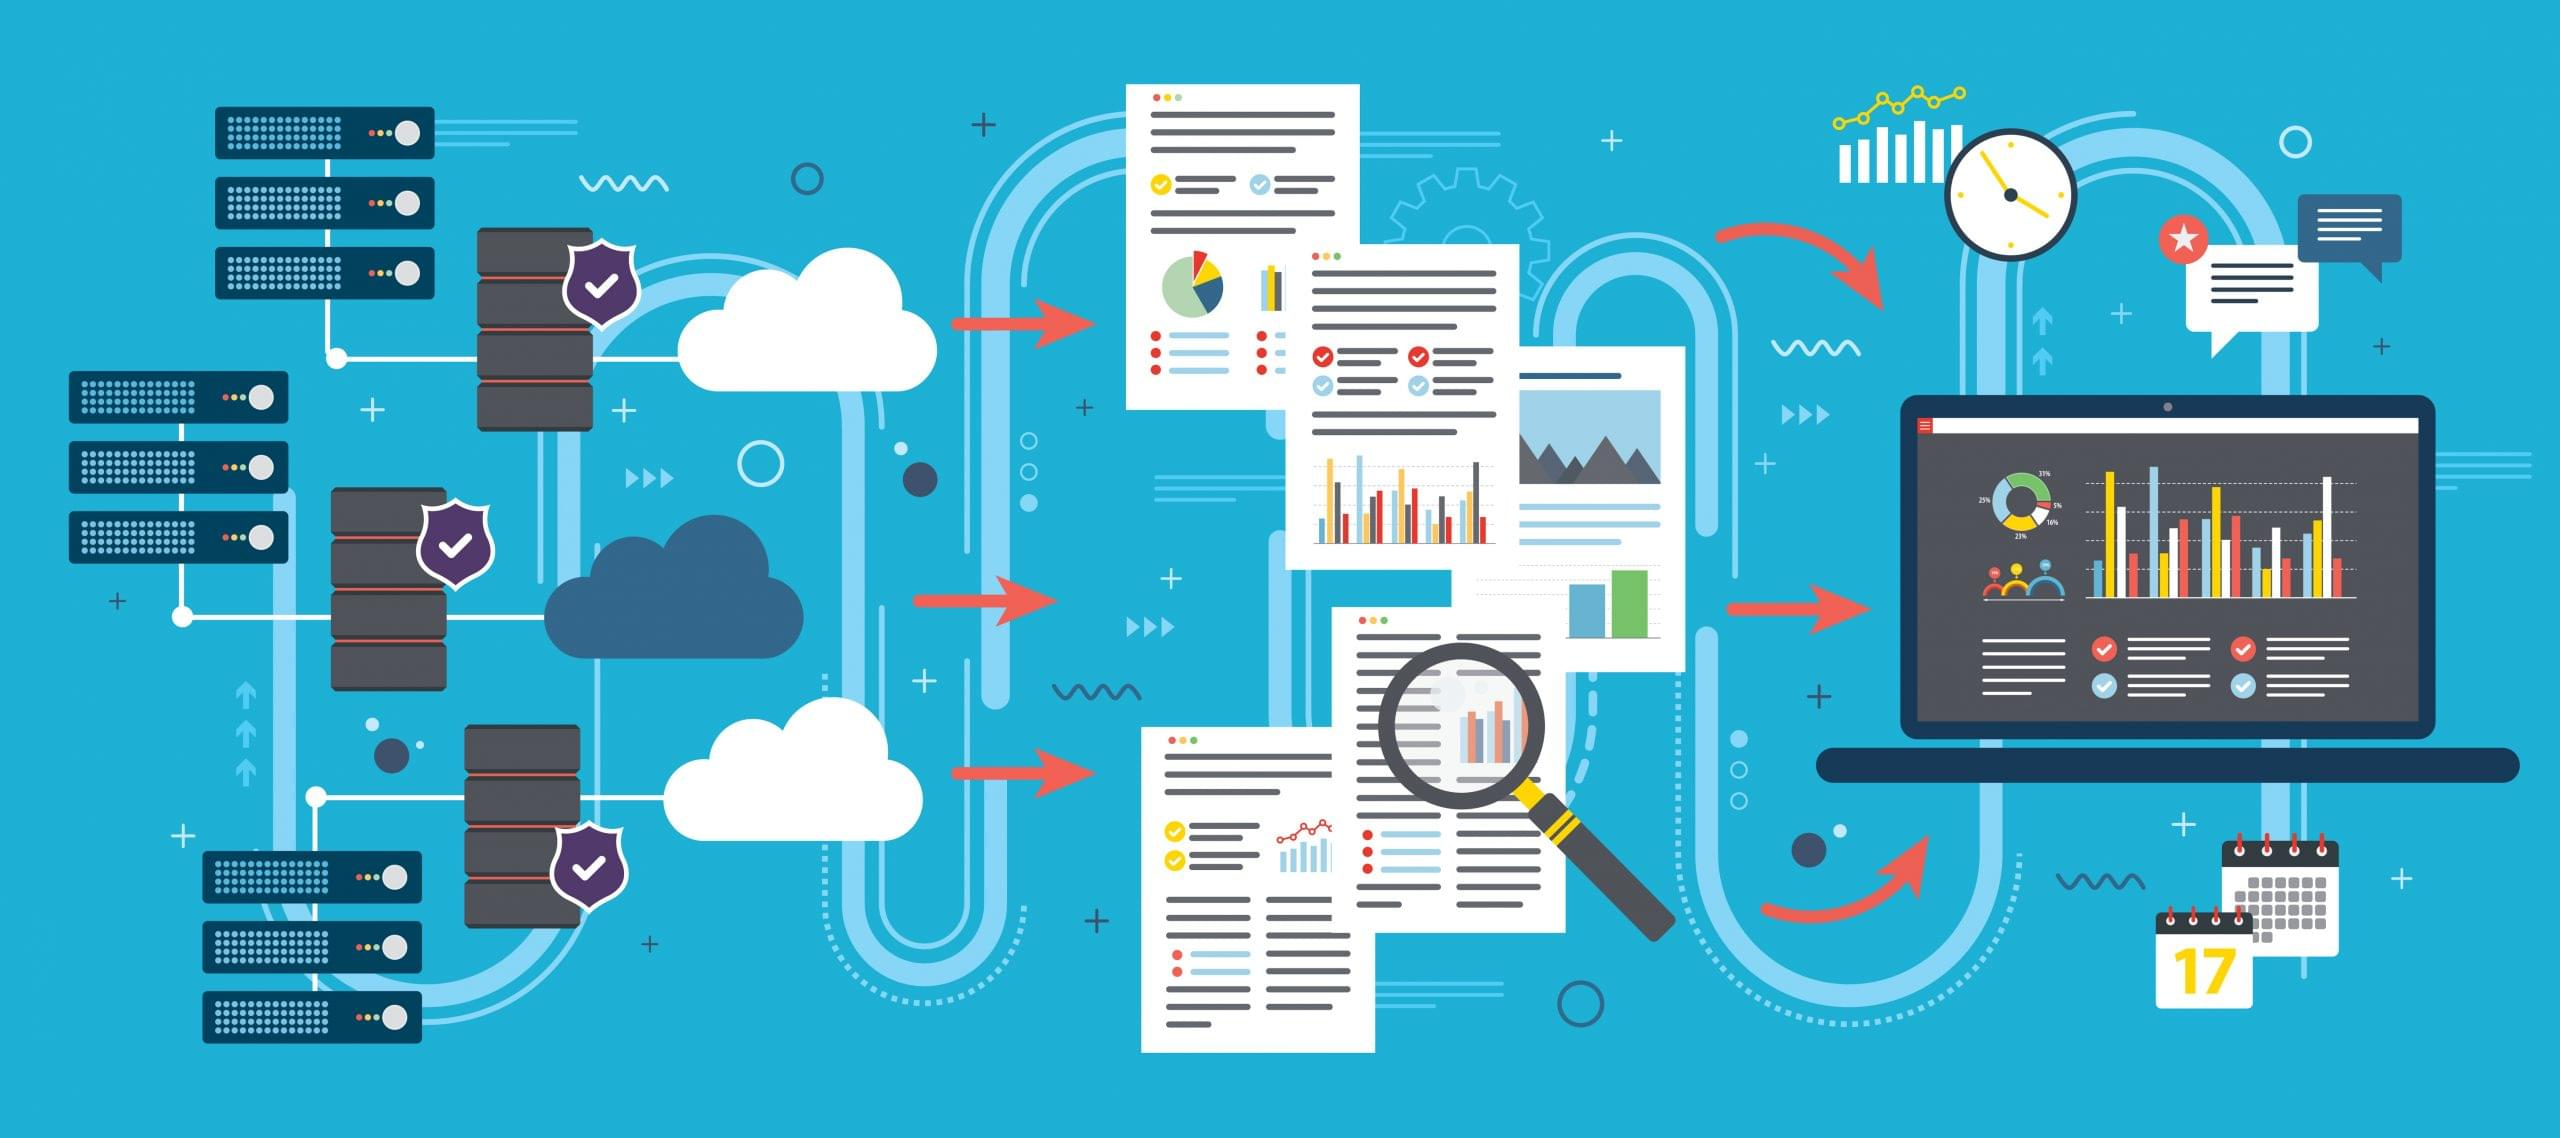
\includegraphics[height=6cm]{images/chap1/BI.jpeg}
    \caption{BI illustration}
    \label{fig:enter-label}
\end{figure}
\subsection*{Key Performance Indicators}
Key Performance Indicators (KPIs) are the critical (key) quantifiable indicators of progress toward an intended result. KPIs provide a focus for strategic and operational improvement, create an analytical basis for decision making and help focus attention on what matters most.

Managing with the use of KPIs includes setting targets (the desired level of performance) and tracking progress against those targets.

Managing with KPIs often means working to improve performance using leading indicators, which are precursors of future success, that will later drive desired impacts indicated with lagging measures.
% \cite{https://www.kpi.org/kpi-basics/}
\subsection{Mobile Development}
Mobile application development is the process of creating software applications that run on a mobile device, and a typical mobile application utilizes a network connection to work with remote computing resources. Hence, the mobile development process involves creating installable software bundles (code, binaries, assets, etc.) , implementing backend services such as data access with an API, and testing the application on target devices.
% \cite{https://aws.amazon.com/mobile/mobile-application-development/#:~:text=Mobile%20application%20development%20is%20the,work%20with%20remote%20computing%20resources.}
\subsection*{Native Development}
Native app development means creating a mobile application that is tailored and dedicated to a specified platform like iOS, or Android. 

Because native applications are built specifically for the operating system, they provide higher user engagement than hybrid apps. Native mobile apps generally perform and look better than their web-based counterparts, which must serve numerous platforms. Furthermore, native mobile applications have access to devise hardware and capabilities, such as sensors and cameras, that are not available via a mobile browser interface alone.
% \cite{https://mdevelopers.com/blog/what-is-a-native-mobile-app-development-}
The two main modern native languages used in the industry are Swift for IOS apps and Kotlin for Android .
\begin{figure}[H]
    \centering
    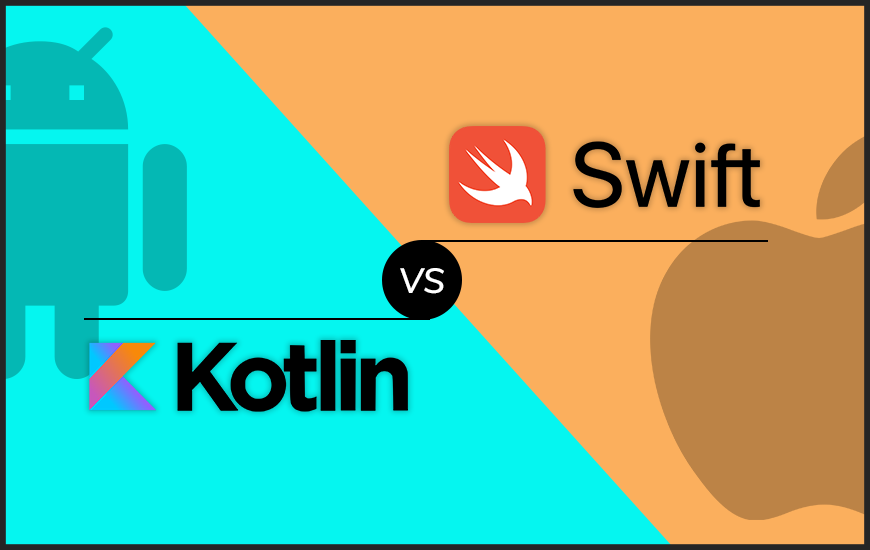
\includegraphics[height=6cm]{images/chap1/kotlin_swift.png}
    \caption{Kotlin\&Swift Logo}
    \label{fig:enter-label}
\end{figure}
\subsection*{Hybrid Development}
You create a hybrid or cross-platform mobile applications from a single codebase. The goal of cross-platform app development is to target different operating systems with one project. You create these apps using cross-platform frameworks, which use platform-specific SDKs (Android SDKs and iOS SDKs) from a unified API. This enables you to easily access the different platform SDKs and libraries.

Private companies create these frameworks. Examples of popular cross-platform frameworks include:

\begin{itemize}
\renewcommand\labelitemi{\textbf{\Huge .}}
\item React Native by Meta. It uses JavaScript as the programming language.
\item Flutter by Google. It uses Dart as the programming language.
\end{itemize}
\begin{figure}[H]
    \centering
    
\includegraphics[height=6cm]{images/chap1/reactNative_Flutter.png}
    \caption{Kotlin\&Swift Logo}
    \label{fig:enter-label}
\end{figure}
\subsection*{The benefit of hybrid application}
% \usepackage{tabularray}
\begin{longtblr}[
  \caption = {Native vs Cross-platform App Developement}
]{
  width = \linewidth,
  colspec = {Q[163]Q[319]Q[460]},
  cells = {c},
  hlines,
  vlines,
}
Feature                     & Cross-Platform App Development                                & Native App Development                                                                      \\
Development Time            & Faster development due to a single codebase                   & Slower development as separate codebases are needed for each platform (Android  iOS)        \\
Development Cost            & Generally lower cost due to code reusability                  & Generally higher cost due to needing separate development teams or expertise                \\
Performance                 & May have slightly slower performance due to abstraction layer & Offers optimal performance as code is tailored to the specific platform                     \\
User Experience (UX)        & May have a less native look and feel                          & Provides a platform-specific UX that feels natural to users                                 \\
Access to Platform Features & May have limitations in accessing all native features         & Full access to all platform features and functionalities                                    \\
Maintenance                 & Easier to maintain due to a single codebase                   & More complex to maintain as separate codebases need updates                                 \\
Learning Curve              & Requires knowledge of cross-platform frameworks               & Requires knowledge of platform-specific languages (e.g., Swift for iOS, Kotlin for Android) \\
Market Reach                & Reaches a wider audience with a single app                    & Reaches platform-specific audiences with separate apps                                      
\end{longtblr}




\vspace{0.5cm}



\section*{Conclusion}
In summary this chapter has given an overview of the internship framework and the organization hosting it. It has defined the projects scope provided examples, from the market explained the project management method chosen talked about the language and software tools used and clarified terms. This examination has laid a groundwork for chapters preparing us for a thorough analysis and implementation of the project. With an understanding of the context project boundaries, methodology employed and necessary tools we are ready to move into the execution phase, with clarity and purpose.

